%卒論概要テンプレート ver. 4.0

\documentclass[uplatex,twocolumn,dvipdfmx]{jsarticle}
\usepackage[top=22mm,bottom=22mm,left=22mm,right=22mm]{geometry}
\setlength{\columnsep}{11mm}
\usepackage[T1]{fontenc}
\usepackage{txfonts}
\usepackage[expert,deluxe]{otf}
\usepackage[dvipdfmx,hiresbb]{graphicx}
\usepackage[dvipdfmx]{hyperref}
\usepackage{pxjahyper}
\usepackage{secdot}





%タイトルと学生番号,名前だけ編集すること
\title{\vspace{-5mm}\fontsize{14pt}{0pt}\selectfont 分散型SNSにおけるユーザの潜在要求分析}
\author{\normalsize プロジェクトマネジメントコース 矢吹研究室 1442037 加藤 健弥}
\date{}
\pagestyle{empty}
\begin{document}
\fontsize{10.5pt}{\baselineskip}\selectfont
\maketitle





%以下が本文
\section{序論}\label{序論}
スマートフォンなどの普及により,手軽にインターネットへの接続が可能になった.そのため,TwitterやFacebookなどの様々なSNS(ソーシャルネットワークサービス)が注目されるようになった.近年ではMastodonという新たなSNSの利用者が増えてきている.

Mastodonとは2016年に公開されたフリーソフトウェアであり,サーバを立てることが出来れば誰でもMastodonを自由に運用することが可能である.そのため,TwitterやFacebookのような利用者が一つのサーバにログインする中央集権型のサービスに対してMastodonでは管理者も設置場所も異なるサーバで運用できる.したがって利用者は自分自身でサーバを選びアカウントを作成してログインする.Mastodonではこのサーバのことを「インスタンス」と呼び,その中で利用者がつぶやきを投稿することを「トゥート」と呼ぶ\cite{Mastodon}.


\section{目的}

TwitterとMastodonのインスタンスをつぶやきを定量的に分析する.その結果からTwitterとは違い,Mastodonではインスタンスごとに話題が異なっているかを調査する.

\section{手法}

Twitter API,Mastodon APIを使用し,Twitterと30のMastodonのインスタンスから1つのインスタンスごとに無作為に100のつぶやきを集める.それにWord2vecを使用し,集めたつぶやきをベクトル化する.その結果をTwitterとMastodonの各インスタンス同士で主成分分析する.


\section{結果}

Twitterと30のMastodonのインスタンスを対象に調査した.図\ref{mstdn}はTwitterと話題が自由なインスタンスであるmstdn.jpのつぶやきをベクトル化し,主成分分析をした結果である.図\ref{ika}はTwitterとスプラトゥーンの話題が中心のインスタンスであるika.queloud.netのつぶやきをベクトル化し,主成分分析した結果である.
\vspace{-1.5zh}
\begin{figure}[h]
\begin{tabular}{cc}
\begin{minipage}{0.5\hsize}
\begin{center}
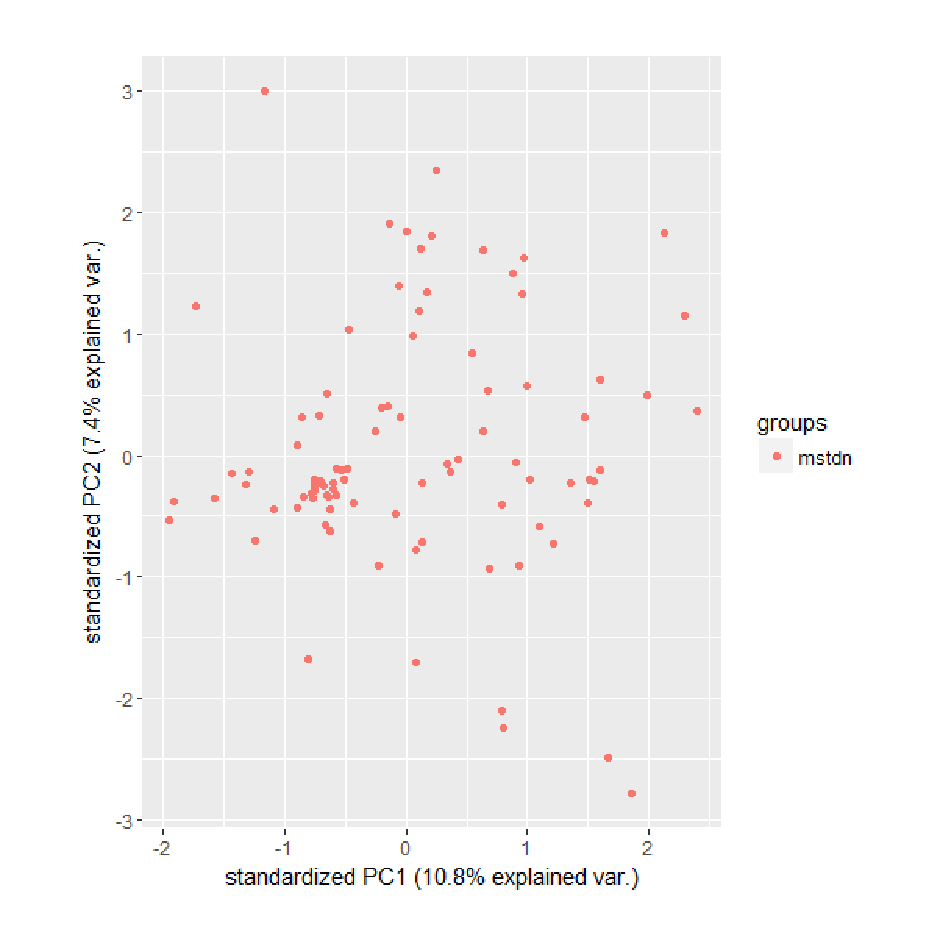
\includegraphics[width=30mm,clip]{mstdn.pdf}
\caption{話題が自由なインスタンス}
\label{mstdn}
\end{center}
\end{minipage}
\begin{minipage}{0.5\hsize}
\begin{center}
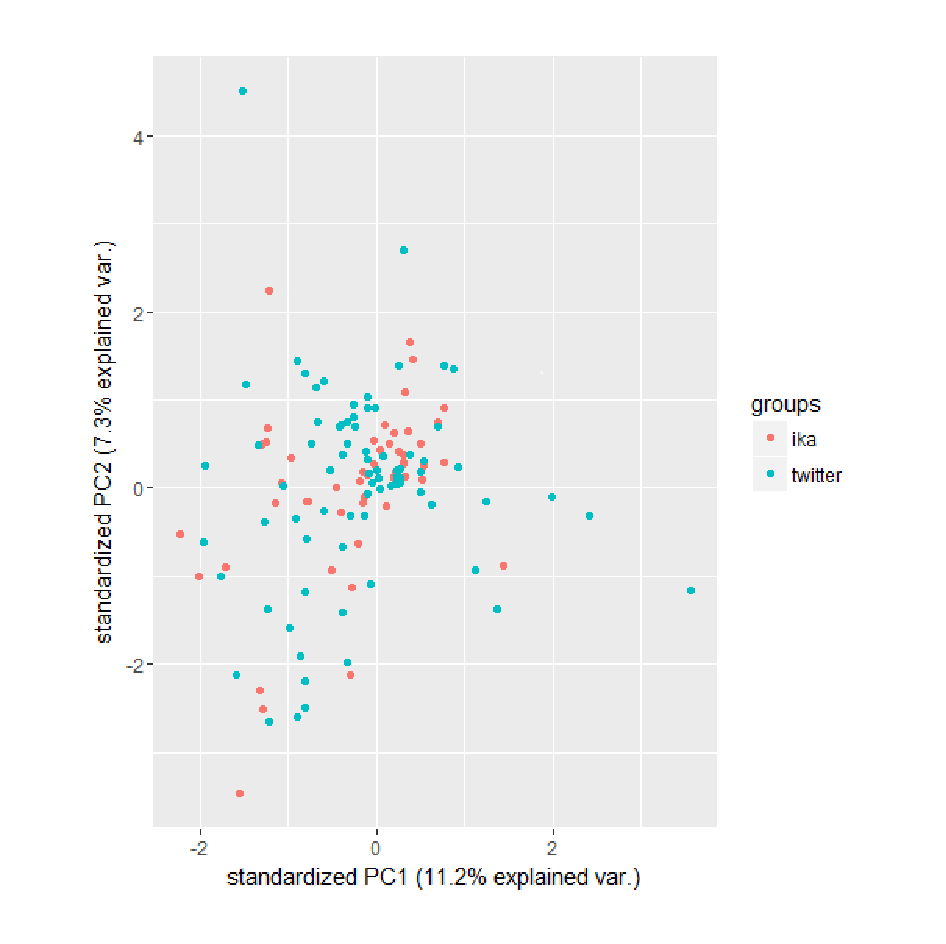
\includegraphics[width=30mm,clip]{ika.pdf}
\caption{スプラトゥーンが話題の中心のインスタンス}
\label{ika}
\end{center} 
\end{minipage}
\end{tabular}
\end{figure}
\vspace{-2.5zh}
\section{考察}

Twitterは話題が幅広いのでつぶやきごとにばらけ,Mastodonのインスタンスは話題が設定されているのでつぶやきがまとまると考えていた.しかし分析した結果,TwitterとMastodonのインスタンスでは違いがみられなかった.そこでTwitterとMastodonのインスタンスのつぶやきを自分の目で確認したが,Twitterは異なる話題,Mastodonのインスタンスでは共通の話題と感じた.しかし私はMastodonのインスタンスで設定されている話題を知っていたため,そのインスタンスが共通の話題であると感じたと考えた.コンピュータもそういったことがわかっているならば研究の結果も変わったと考える.


\section{結論}

TwitterとMastodonの各インスタンスのつぶやきを定量的に分析した.人間の目でみて共通の話題をしていると感じたインスタンスであってもコンピュータが判別することへの精度は低いとわかった.
今後はMastodonのインスタンスに設定されている話題をコンピュータに勉強させているならば精度の高い判別ができると期待される.

\bibliographystyle{junsrt}
\bibliography{biblio}%「biblio.bib」というファイルが必要.

\end{document}